In this section, I describe the salient aspects of the Albuquerque pilot.
The project is operated by Token Ibis, an all-volunteer organization created in 2019 in Albuquerque for the sole purpose of operating the pilot.
While most of its long-term funding is provided by its board of directors, it accepts donations under its 501(c)(3) status.
Its primary service is the development and maintenance of a web application that facilitates interactions between individuals and organizations according to the UBP model.
The application software, a combination of a Django backend and ReactJS frontend, is free and open-source under the GPL-3.0 license.
Although the platform maintains some private data such as private messages and user credentials, all data used in this study is publicly available through the platform's GraphQL endpoint\footnote{\url{https://api.app.tokenibis.org/graphql/}} and permitted for research use under the organization's user agreement\footnote{\url{https://tokenibis.org/user-agreement-and-privacy-policy/}}.

Access to the application is available to all users who can (1) verify a phone number and (2) log in using a Google, Facebook, or Microsoft OAuth account.
While it is technically possible for one user to open multiple accounts in violation of the platform policy, a cursory inspection of the user pool did not reveal any overt attempts to abuse the platform in this way.
Within the application, Figure~\ref{fig:application} shows three sample screenshots of the core user experience.
Users begin on the home page, which displays their current balance.
By navigating to the nonprofit page, users can browse the list of available organizations and read a short description of their mission.
Once a user selects and allocates funds, then a donation is recorded to the public ledger.
As long as the user remains active on the application, the platform automatically additional funds at the same time every week.

\begin{figure}[H]
  \centering
  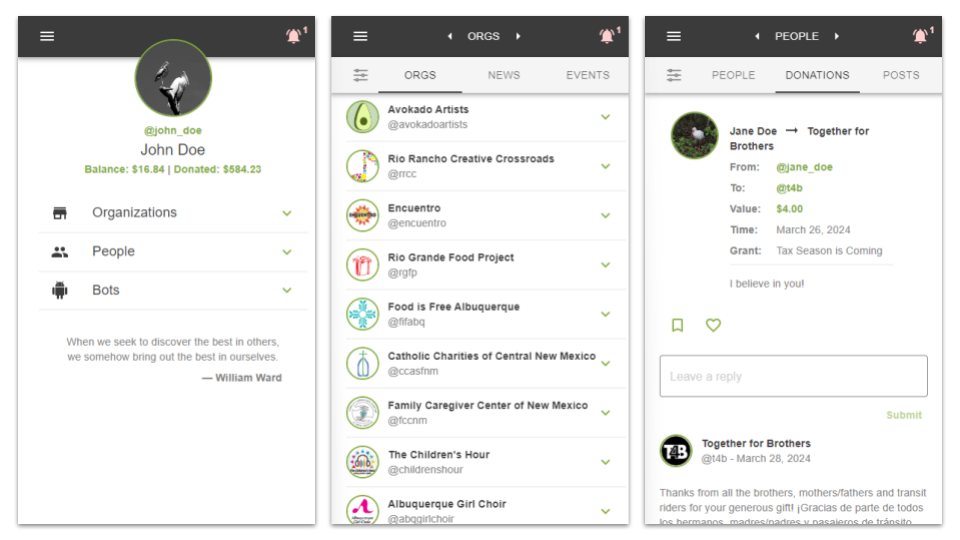
\includegraphics[width=\linewidth]{figures/application}
  \caption{Sample screenshots of the Albuquerque pilot web application (left: home screen, middle: organization list, right: donation)}
  \Description{The three screenshots convey a simple but functional Web 2.0 application.}
  \label{fig:application}
\end{figure}

In addition to the core donation workflow, the platform also supports several auxiliary activities. 

\begin{itemize}
  \item \textbf{Communication}: Users can engage in rudimentary social-media-like interactions through posts, comments, ``likes'', and private messages.
  \item \textbf{Games}: Users can participate in a set of public games---administered by on-app ``bots''---to earn more money to donate. For example, a ``vocabulary bot'' periodically rewards users who include vocabular in their donation messages that has not been used before.
  \item \textbf{Grants}: Users can deposit their own money, called grants, into the platform. These contributions are evenly distributed among all active users.
\end{itemize}

Organizations have accounts that they can use to engage with users and other organizations.
The level of engagement of each organization determines its place on the list and, therefore, its exposure to new donors.
Finally, the design of the Albuquerque pilot explicitly maintains two invariants that are relevant to this study.

\begin{itemize}

  \item \textbf{Individual Influence}: All users have equal opportunity to become influential nodes regardless.
In particular, the platform does not allow users to deposit money into their accounts.
The only mechanism for users to supplement their influence is to be active on the platform.

  \item \textbf{Organizational Exposure}: All organizations have equal opportunity to become influential nodes.
In particular, the application does not encourage users to donate to any organization based on mission type, size, or other intrinsic factors.
The only mechanism for organizations to supplement their influence is to be active on the platform.

\end{itemize}

As of May 9th, 2024, this model has facilitated the distribution of \$145,641 across 13,812 donations by 702 users to 59 organizations.
The bulk of this activity occurred over approximatley four years.
Figure~\ref{fig:graph} provides a complete picture of the network data used in this study.
Since the launch of the project, two organizations were removed for administrative reasons.
I removed the \$667.22 worth of donation activity associated with these two nonprofits from Figure~\ref{fig:graph} and all subsequent analysis.

\begin{figure}[H]
  \centering
  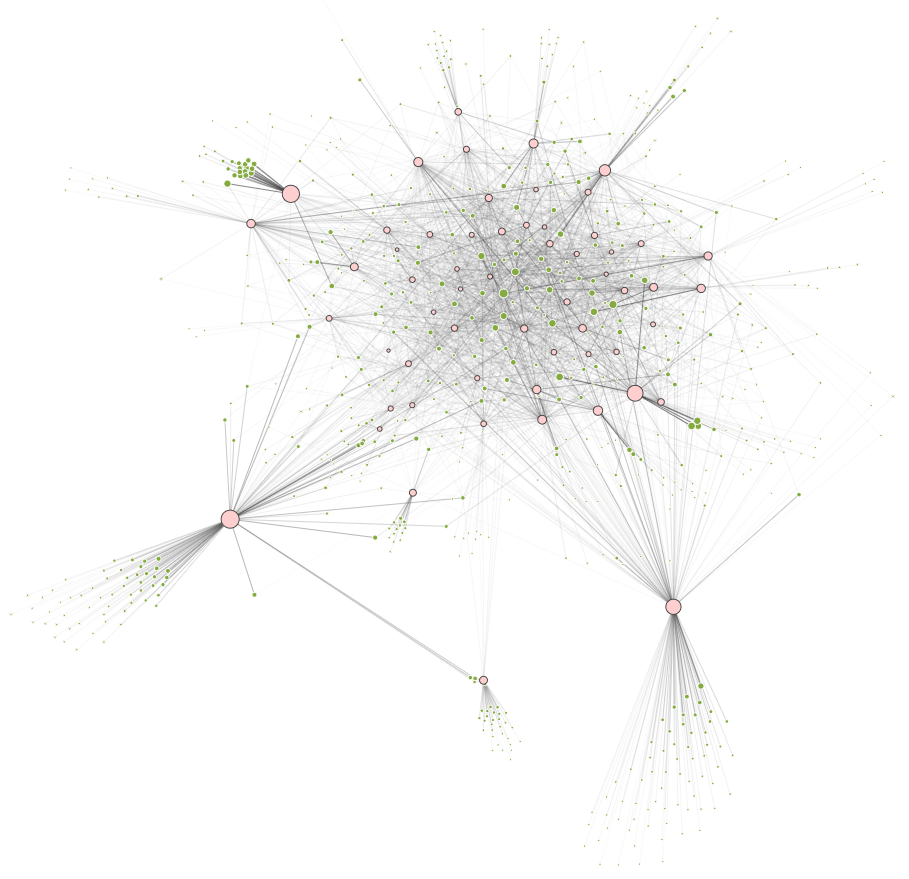
\includegraphics[width=\linewidth]{figures/network}
  \caption{Network visual of aggregate donation flow from individuals (green) to organizations (pink). The area of circles and the width and opacity of edges correspond to aggregate amounts.}
  \Description{The network is characterized by one densely connected main subgraph of individuals and organizations and several periphery hubs with one organization at the center of each hub.}
  \label{fig:graph}
\end{figure}
